\chapter{CONTEXTUALIZAÇÃO DA INSTITUIÇÃO}
\label{chap:contex}

Este Capítulo trata de dados históricos da Universidade Tecnológica Federal do Paraná (UTFPR), o contexto da instituição no estado do Paraná e a instauração do curso de Engenharia Eletrônica no Câmpus da cidade de Toledo.

\section{HISTÓRICO DA UNIVERSIDADE TECNOLÓGICA FEDERAL DO PARANÁ}
\label{sec:hist}

A história da UTFPR teve início no início século passado. Sua trajetória começou com a criação das Escolas de Aprendizes Artífices em várias capitais do país, pelo então presidente Nilo Peçanha, em 23 de setembro de 1909. No Paraná, a escola foi inaugurada no dia 16 de janeiro de 1910, em um prédio da Praça Carlos Gomes em Curitiba. O ensino era destinado a garotos de camadas menos favorecidas da sociedade, chamados de ``desprovidos da sorte''. Pela manhã, esses meninos recebiam conhecimentos elementares (primário) e, de tarde, aprendiam ofícios nas áreas de alfaiataria, sapataria, marcenaria e serralheria. Inicialmente, havia 45 estudantes matriculados na escola, que, logo em seguida, instalou seções de Pintura Decorativa e Escultura Ornamental. Aos poucos, a escola cresceu e o número de estudantes aumentou, fazendo com que se procurasse uma sede maior. Então, em 1936, a Instituição foi transferida para a Avenida Sete de Setembro com a Rua Desembargador Westphalen, onde permanece até hoje.

O ensino tornou-se cada vez mais profissional até que, no ano seguinte (1937), a escola começou a ministrar o ensino de 1º grau, sendo denominada Liceu Industrial do Paraná. Cinco anos depois (1942), a organização do ensino industrial foi realizada em todo o país. A partir disso, o ensino passou a ser ministrado em dois ciclos. No primeiro, havia o ensino industrial básico, o de mestria e o artesanal. No segundo, o técnico e o pedagógico. Com a reforma, foi instituída a rede federal de instituições de ensino industrial e o Liceu passou a chamar-se Escola Técnica de Curitiba. Em 1943, tiveram início os primeiros cursos técnicos: Construção de Máquinas e Motores, Edificações, Desenho Técnico e Decoração de Interiores. Antes dividido em ramos diferentes, em 1959, o ensino técnico no Brasil foi unificado pela legislação em vigor.

A escola ganhou, assim, maior autonomia e passou a chamar-se Escola Técnica Federal do Paraná. Em 1974, foram implantados os primeiros cursos de curta duração de Engenharia de Operação (Construção Civil e Elétrica). Quatro anos depois (1978), a Instituição foi transformada em Centro Federal de Educação Tecnológica do Paraná (CEFET-PR), passando a ministrar cursos de graduação plena. A partir da implantação dos cursos superiores, deu-se início ao processo de “maioridade” da Instituição, que avançaria, nas décadas de 80 e 90, com a criação dos Programas de Pós-Graduação. Em 1990, o Programa de Expansão e Melhoria do Ensino Técnico fez com que o CEFET-PR se expandisse para o interior do Paraná, onde implantou unidades. Com a Lei de Diretrizes e Bases da Educação (LDBE) \cite{Lei:9394:1996}, que não permitia mais a oferta dos cursos técnicos integrados, a Instituição, tradicional na oferta desses cursos, decidiu implantar o Ensino Médio e cursos de Tecnologia. Em 1998, em virtude das legislações complementares à LDBE, a diretoria do então CEFET-PR tomou uma decisão ainda mais ousada: criou um projeto de transformação da Instituição em Universidade Tecnológica.

\nomenclature[A]{CEFET-PR}{Centro Federal de Educação Tecnológica do Paraná}
\nomenclature[A]{LDBE}{Lei de Diretrizes e Bases da Educação}

Após sete anos de preparo e o aval do governo federal, o projeto tornou-se lei no dia 7 de outubro de 2005. O CEFET-PR, então, passou a ser a Universidade Tecnológica Federal do Paraná (UTFPR) \cite{Lei:11.184:2005} – a primeira especializada do Brasil. Atualmente, a Universidade Tecnológica conta com 13 câmpus, distribuídos nas cidades de Apucarana, Campo Mourão, Cornélio Procópio, Curitiba, Dois Vizinhos, Francisco Beltrão, Guarapuava, Londrina,  Medianeira, Pato Branco, Ponta Grossa, Santa Helena e Toledo, conforme mostra a \autoref{fig:13campi}. O Quadro 1 apresenta, de forma resumida, as diferentes denominações que a instituição teve ao longo do tempo.

\nomenclature[A]{UTFPR}{Universidade Tecnológica Federal do Paraná}

    \begin{figure}[!htb]
        \centering
        \caption[Localização dos 13 Câmpus da UTFPR]{Localização dos 13 Câmpus da UTFPR no estado do Paraná}
        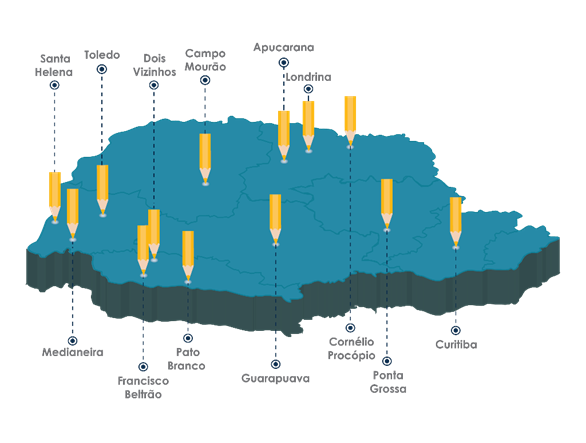
\includegraphics[width=0.7\textwidth]{Caps/Figs/campus_utfpr.png}
        \fonte{\utf}
        \label{fig:13campi}
    \end{figure}
    
    \begin{quadro}
        \centering
        \caption[Diferentes denominações da UTFPR]{As diferentes denominações da UTFPR ao longo de sua existência}
        \pgfplotstabletypeset[%
		every head row/.style={before row=\toprule,after row=\midrule},
		every last row/.style={after row=\bottomrule},
		columns/Fruit/.style={string type},
		columns/Animal/.style={string type}
	    ]%
	    {Caps/Quadros/denominacoes_utfpr.csv}
        \label{qua:denomi}
    \end{quadro}